
% this file is called up by thesis.tex
% content in this file will be fed into the main document
%----------------------- introduction file header -----------------------
%%%%%%%%%%%%%%%%%%%%%%%%%%%%%%%%%%%%%%%%%%%%%%%%%%%%%%%%%%%%%%%%%%%%%%%%%
%  Capítulo 1: Introducción- DEFINIR OBJETIVOS DE LA TESIS              %
%%%%%%%%%%%%%%%%%%%%%%%%%%%%%%%%%%%%%%%%%%%%%%%%%%%%%%%%%%%%%%%%%%%%%%%%%

\chapter{Análisis de nuevas}

Para las gráficas del trabajo se utilizaron diferentes colores para caracterizar las influencias de un idioma, además en cada gráfica se especifica los idiomas que intervienen y para su mejor lectura se utilizaron abreviaciones. Los colores y abreviaciones de cada idioma son:

\hfill\break

inglés   $\rightarrow$  EN $\rightarrow$  azul

francés  $\rightarrow$  FR $\rightarrow$  amarillo

alemán   $\rightarrow$  GE $\rightarrow$  violeta

italiano $\rightarrow$  IT $\rightarrow$  verde

español  $\rightarrow$  SP $\rightarrow$  guinda

\hfill\break

Para las gráficas comparando la influencia entre dos idiomas, la primera abreviación que aparezca en la leyenda será el idioma origen de los préstamos, y la segunda corresponderá al idioma receptor, el color de cada una indicará el idioma origen. Por ejemplo, si se grafica la influencia entre el inglés y el francés,  la leyenda EN-FR seran los préstamos que van del inglés al francés y se graficarán con color azul,  en cambio la leyenda FR-EN son los préstamos que van en sentido contrario, del francés al inglés en color amarillo.  

\hfill\break

En todas las gráficas, el eje horizontal está representado por los años del conjunto de búsqueda 1900-2009,  mientras que en el eje vertical se presenta la medición de la influencia ya sea en cantidad o en frecuencia. 



\newpage

\section{Palabras nuevas entre dos idiomas}

Se estima la influencia por cantidad en los  préstamos nuevos que entraron a un idioma receptor provenientes de un idioma origen; el año de entrada del préstamo es aquel donde apareció en la lista de las cinco mil palabras más usadas del receptor por primera vez. 

La motivación de cuantificar así la influencia es notar si algún idioma ha crecido más en los demás durante el siglo XX y la primera década del siglo XXI, y asociar los crecimientos a eventos políticos, culturales, históricos o sociales. 

Para disposición del lector, se puede consultar la lista de los préstamos nuevos de un idioma a otro, en la referencia \cite{prestamos_nuevos}.  Las instrucciones de cómo se deben interpretar las palabras se encuentran en el apéndice 1. 

Analizar el contenido de las listas, permitirá hacer conclusiones sobre la causa de las migraciones. 



\subsection{Inglés y Francés}


\begin{figure}[h!]
	\centering
	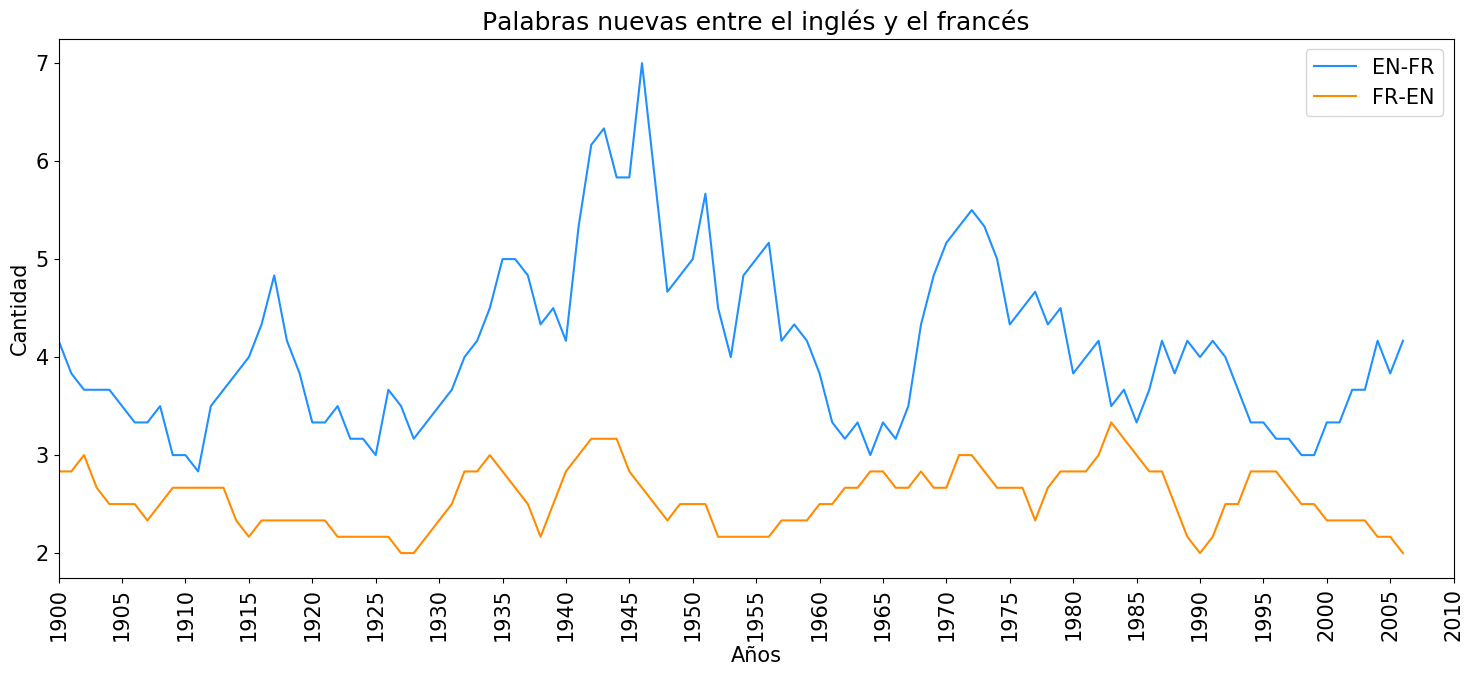
\includegraphics[scale=.38]{Cap_2/NC_1_S2_EN.png}
	\label{NC_EF}
	\caption{}
\end{figure}


La primera conclusión tras ver la gráfica, es que el inglés aportó mayor cantidad de palabras al francés que el caso contrario, los aportes no fueron constantes, sino que existieron períodos de tiempo 1910-1920, 1935-1960, 1965-1975 donde la migración fue más evidente (periodos donde hay picos en las trazas).  En el contexto histórico, en los primeros dos periodos ocurrieron las guerras mundiales, donde intervinieron países de habla inglesa y francesa.   Este argumento puede ser comprobado al consultar la lista de préstamos nuevos del inglés al francés; específicamente para los años 1944 y 1945, entre el contenido de la lista se encuentran \textit{Churchill}, \textit{territories,} \textit{nazis} y \textit{catastrophe} palabras que están relacionadas con la segunda guerra mundial por los años de aparición. Para el último periodo,  el contenido de la lista tiene palabras como \textit{Nixon} \textit{dollar} y \textit{Johnson}; dos de estas palabras aluden a apellidos que fueron importantes en el periodo, posiblemente ya existían estas palabras en el francés, pero hasta los años entre 1965 y 1975 fue que cobraron notoriedad por algún personaje que fue importante en esa época,  específicamente Lyndon B. Johnson y Richard Nixon, presidentes de Estados Unidos entre 1963-1969 y 1969-1974 respectivamente.

Los periodos más prolongados donde existieron aportes del francés al inglés,  ocurrieron entre 1930-1950 y 1975-1990,  sin embargo la lista de los préstamos no muestra palabras que se puedan asociar a un evento,   pero si hay palabras comunes en el inglés y el programa las detecto como provenientes del francés, como lo son \textit{diagnostic,} \textit{clients,} \textit{placement,} \textit{adaptation,} \textit{diffusion,} \textit{amplitude,} entre otras, estas son palabras que el programa clasificó como de origen francés, ya que fue el primer idioma donde tuvieron relevancia,  y que después las retomo el inglés. Esta propuesta puede sugerir que en años anteriores el francés era rico o basto de palabras de otros idiomas, o que los idiomas utilizaban al francés para poder llegar a más conjuntos. En un análisis posterior, se mostrará el uso que tenía el francés en el siglo XIX, comparado con el que tuvo en el siglo XX. 

De manera general para todos los idiomas, existirán casos donde las préstamos de un idioma en otro serán nombres, apellidos, ciudades o países, como el caso que ya se comentó anteriormente. Estas palabras pueden mostrar un evento histórico al estar relacionada con personajes o lugares del evento y también por la fecha en la que aparecieron. 


\newpage


\subsection{Inglés y Alemán}


\begin{figure}[h!]
	\centering
	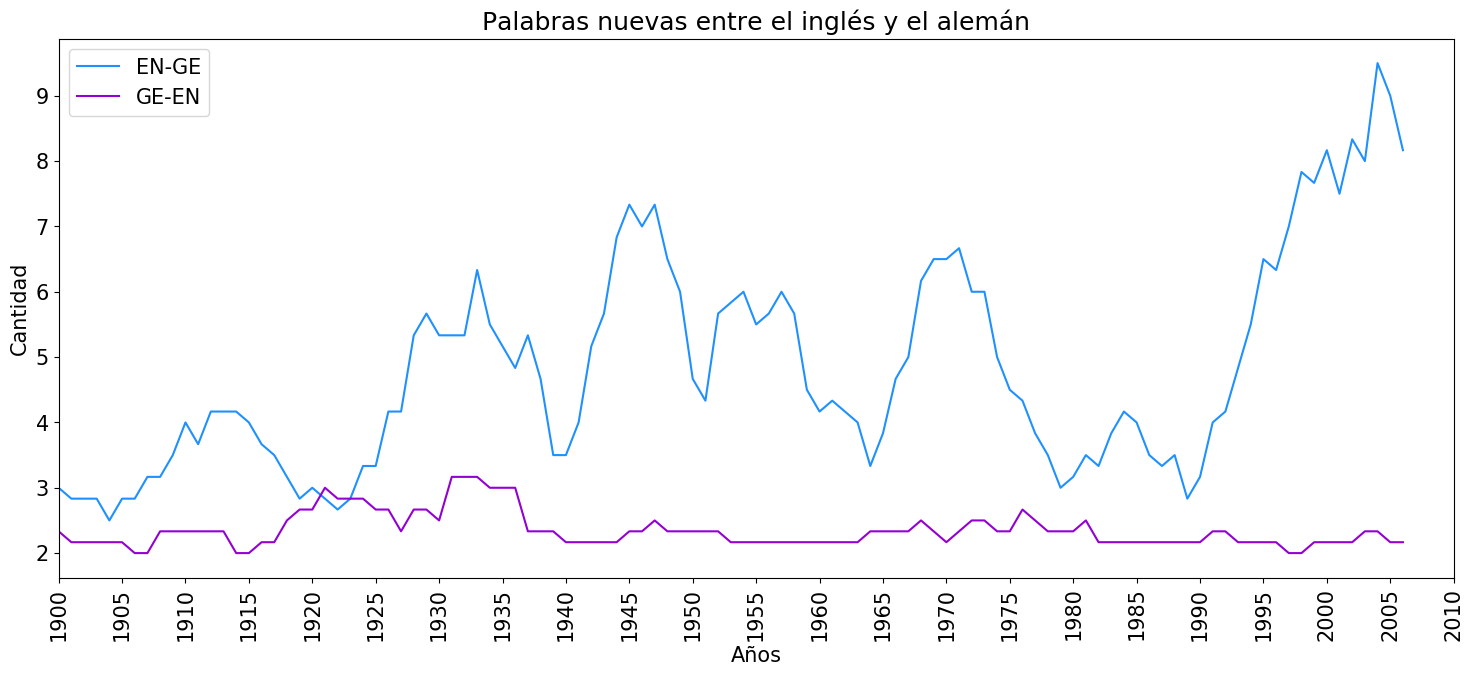
\includegraphics[scale=.38]{Cap_2/NC_2_S2_EN.png}
	\label{NC_EG}
	\caption{}
\end{figure}


El mayor aporte ocurrió del inglés al alemán, hay muchos periodos donde la cantidad de préstamos sobresalen, el primero entre 1920 y 1935,  el inglés aportó  palabras como \textit{economic} (1929), \textit{depression} (1931),  \textit{investment} (1933), \textit{Roosevelt} (1935) , que pertenecen al campo semántico de la gran depresión, evento que tuvo origen en los Estados Unidos  con consecuencias en muchos países, en este caso en Alemania, ya que fue uno de los motivos para que se originara la segunda guerra mundial.  Durante los años de la segunda guerra las palabras encontradas fueron \textit{Churchill} (1940), \textit{Stalin} (1943), \textit{nazi} (1945),  \textit{justice} (1947),  las cuales si están relacionadas con el suceso.  Finalmente alrededor de 1990, el inglés ha aportado de manera creciente más palabras al alemán, el desarrollo de la tecnología y la globalización son responsables de esta tendencia al estar involucradas palabras como \textit{standards} (1933), \textit{market} (1994),  \textit{internet} (1996), \textit{online} (1988). 

Para el préstamo en sentido inverso, el alemán presentó muchos años donde no llevó palabras de él hacia el inglés,  pero las pocas que lo hicieron muestran información histórica, como \textit{Lenin} (1931), \textit{Marx} y \textit{Hitler} (1934),  \textit{reich} (1939) y  \textit{Mao} (1967),  en alusión a la segunda guerra mundial y a la revolución china que ocurrió durante la guerra fría.

La relación entre el inglés y el alemán en el ámbito de préstamos se vio marcada por palabras que van de un lado a otro con relaciones a un hecho histórico que involucró a países cuyas lenguas son estos idiomas.  Por el momento se está haciendo evidente que los eventos políticos o históricos si permiten que exista una migración de palabras entre idiomas. 

\newpage
\subsection{Inglés e Italiano}

\begin{figure}[h!]
	\centering
	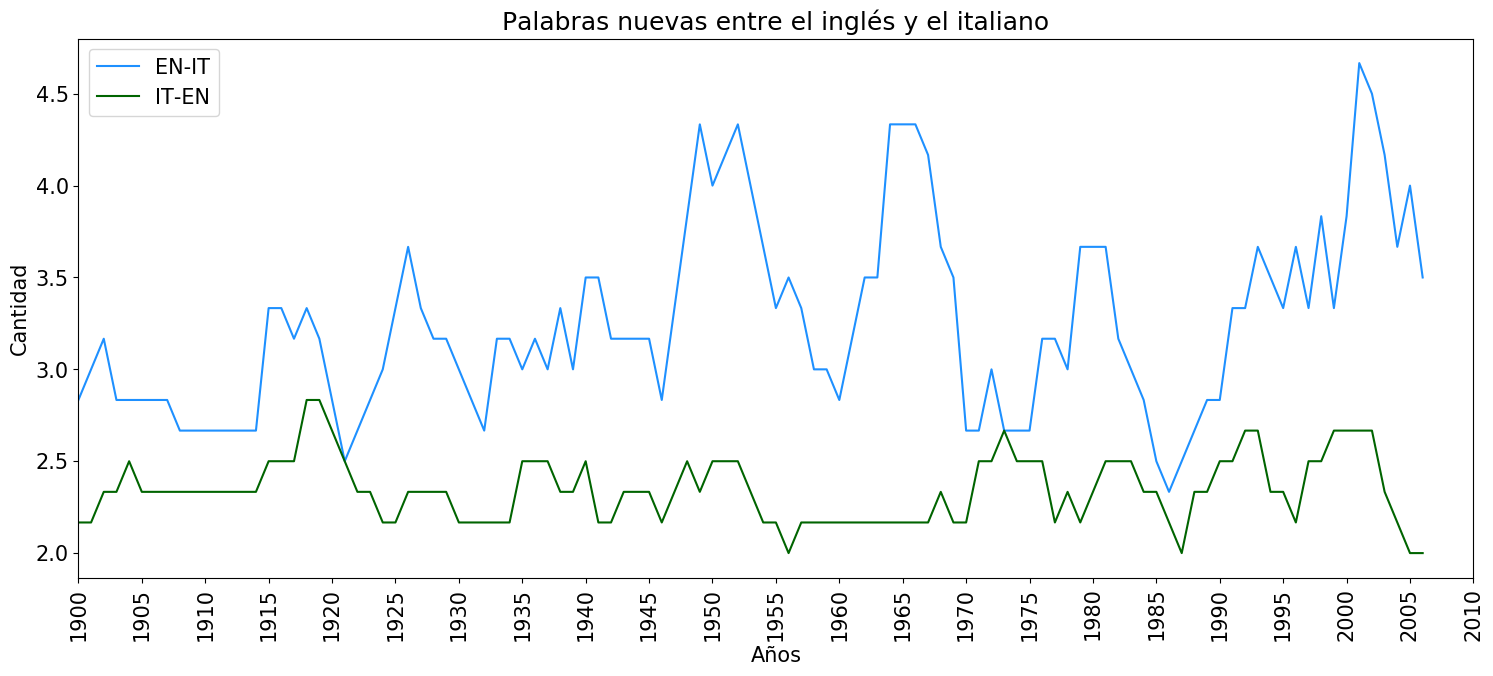
\includegraphics[scale=.38]{Cap_2/NC_3_S2_EN.png}
	\label{NC_EI}
	\caption{}
\end{figure}

El sentido de mayor cantidad de migraciones ocurrió del inglés hacia el italiano, donde es evidente periodos alrededor de las guerras como en el caso de las migraciones del inglés hacia el francés y el alemán,  nuevamente palabras como \textit{Roosevelt} (1941) o \textit{Stalin} (1949) son de carácter histórico; \textit{Mussolini} (1935)  presente en las migraciones del italiano al inglés es otro ejemplo de la relación de la guerra con estos idiomas y en esos años.A pesar de que la gráfica del inglés al italiano se vea favorecida en cantidad, muchas de las palabras no se consideraron préstamos de carácter histórico, ya que son palabras que no portan información que las ligue a un evento, sin embargo se asentaron en el italiano y han sido usadas en al menos dos años dentro de la lista de cinco mil. 

Los préstamos del italiano en el inglés, fueron nulos durante muchos años, los pocos en los que existieron, las palabras no se lograron  ligar a un suceso que explicara el por qué ocurrieron las migraciones,  salvo el ejemplo ya mencionado.

\newpage


\subsection{Inglés y Español}
\begin{figure}[h!]
	\centering
	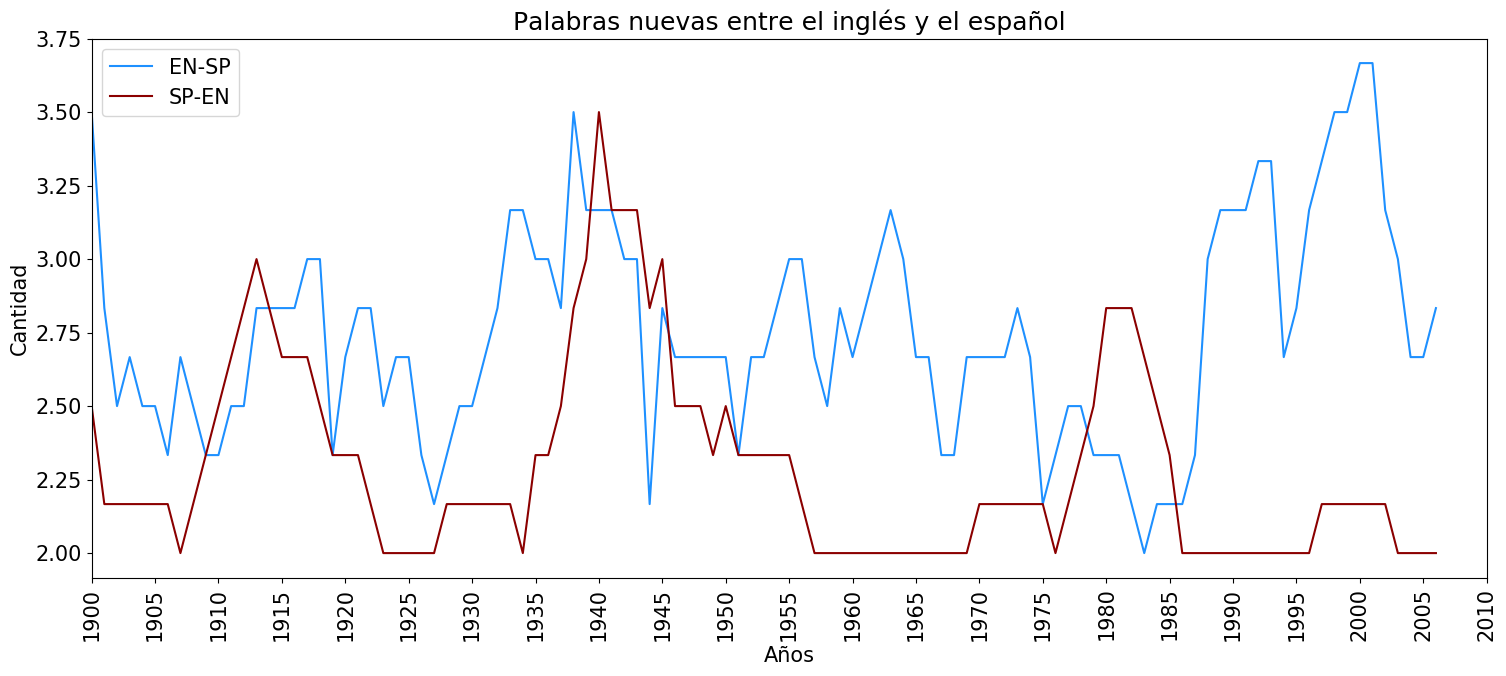
\includegraphics[scale=.38]{Cap_2/NC_4_S2_EN.png}
	\label{NC_ES}
	\caption{}
\end{figure}

El español ha sido el único idioma que ha aportado en algunas épocas igual cantidad de palabras al inglés como el inglés aportó al español,  en los demás idiomas la tendencia era que el inglés aportaba más que los demás a él.  Las dos gráficas muestran similar crecimiento en periodos de la primera mitad de siglo,  como de 1905 - 1925, y en 1935-1950.  En la segunda mitad del siglo XX,  se presentaron mayor cantidad de préstamos del inglés al español, y el sentido opuesto tuvo muchos periodos donde no aportó alguna palabra,  siendo el más relevante entre 1975 y 1985. 

Entre los préstamos encontrados en el sentido inglés-español, se encuentran \textit{oil} (1931), \textit{standard} (1933),  referentes a la compañía de petróleos de Standart Oil de John D.  Rockefeller,  \textit{unesco} (1955); de estas palabras es curioso que aparecieron en el español tras un letargo de años en el que eran importantes en el inglés,  por ejemplo, la empresa Standard Oil, cobró relevancia por ser el primer gran monopolio entre finales del siglo XIX y su disolución en 1911,  transcurrieron cerca de treinta años para que el español se comenzará a hablar acerca de ello. Un letargo menos extenso ocurrió con la palabra Unesco, esta organización se fundó diez años antes (1945)  de que entrara a la lista de español.  

Conforme se avanza en los años, aparecen palabras como \textit{Kennedy} (1961), \textit{nuclear} (1962) (sin acento al provenir del ingles), \textit{Nixon} (1972),  \textit{Bush} (1990), \textit{internet} (1996) e  \textit{Irak} (2003),  de este conjunto, tres son apellidos de presidentes de los Estados Unidos, pero no hay un desfase prolongado entre la fecha de relevancia en el conjunto original (para este caso los años en que fueron presidentes) y el año donde aparecen en el receptor. Palabras como nuclear e Irak, también son de carácter histórico aludiendo a los conflictos bélicos que se dieron alrededor de su fecha de aparición, igualmente no tuvieron un desfase de años, mientras que internet alude al desarrollo de esta herramienta. 


Por parte de los préstamos que van del español hacia el inglés,  se lograron ligar palabras al campo de la medicina,  en el año de 1943 aparecieron las palabras \textit{virus} y \textit{anemia}, años antes en 1934 George Richards Minot, Parry Murphy y George Hoiyt Whipple, habían recibido el premio nobel de medicina por su descubrimiento de la terapia de hígado en las anemias.  También migraron nombres de países como \textit{Chile} (1920), \textit{Argentina} (1941),  \textit{Venezuela} (1942).

La conclusión general  de estos argumentos es que la “velocidad” con la que se transmiten palabras de un idioma a otro,  ha ido en aumento conforme se avanza en el tiempo, permitiendo que cada vez sea más inmediata, además las palabras ligadas a sucesos históricos no son solo en el ámbito político, sino también al desarrollo científico y tecnológico. 


\hfill\break

\subsection{Francés y Alemán}

\begin{figure}[h!]
	\centering
	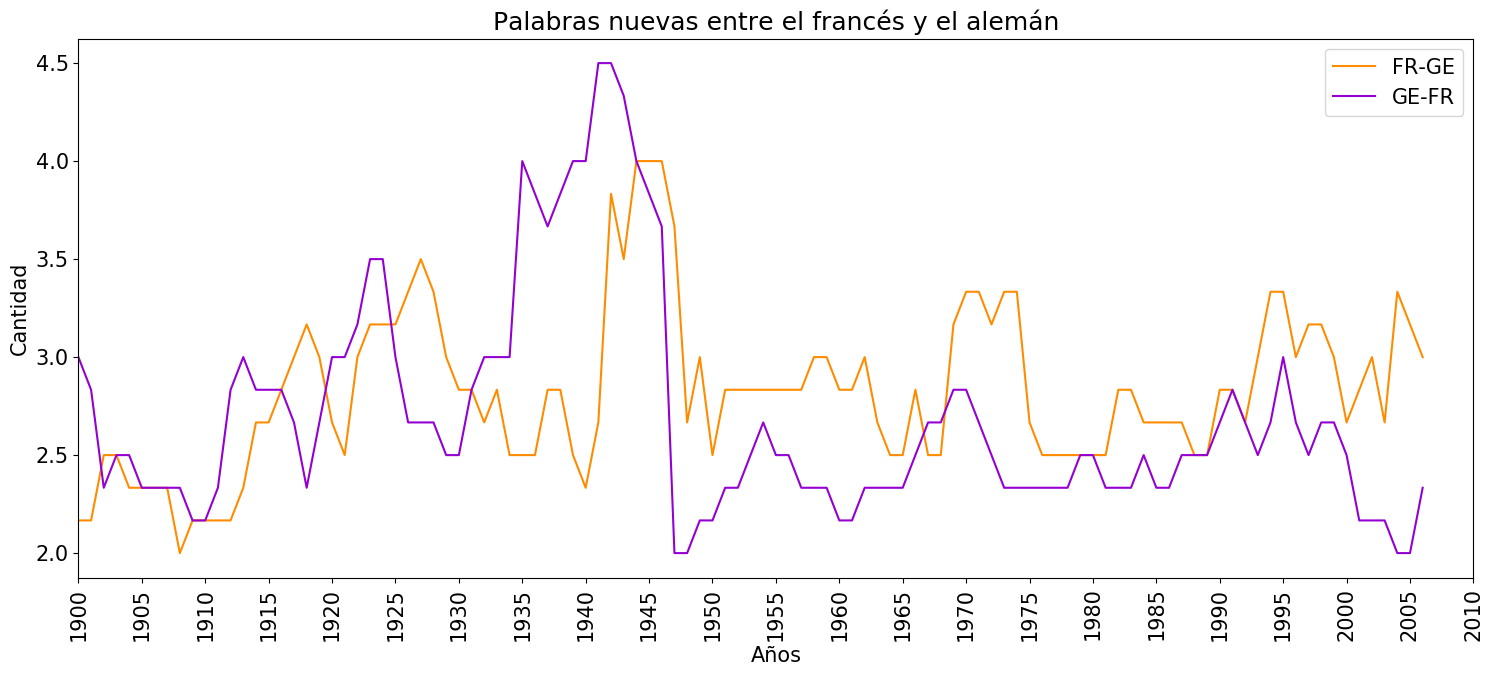
\includegraphics[scale=.38]{Cap_2/NC_2_S2_FR.png}
	\label{NC_FG}
	\caption{}
\end{figure}


Las aportaciones entre ambos idiomas han sido equitativas,  teniendo un comportamiento similar en diferentes plazos, el alemán logra su punto más alto entre 1940, mientras que el francés lo hace  en 1945.  Las primeras dos clafisicaciones que se hicieron para los préstamos que van del francés al alemán son a partir de términos políticos como \textit{diplomatie} (1917), \textit{bourgeoisie} (1919),  \textit{guerre} (1925),  \textit{empire} (1937), y por nombres de  países como \textit{Ukraine} (1918),  \textit{Allemagne} y \textit{Russie} (1925) y \textit{Vietnam} (1965).  Dentro de un entorno histórico,  ambas clasificaciones pueden simplificarse en una, ya que para los años de aparición, es posible que en una misma oración o párrafo coexistan palabras de las dos clasificaciones.  La última clasificación hecha para esté sentido de migración son términos del campo semántico del desarrollo tecnológico como \textit{technologie} (1969),  \textit{innovation} (1996), \textit{informations} (1997),  \textit{mobile} y \textit{communication} (2007).  Estas palabras también tienen en común que su origen es el inglés y que aparecieron en la segunda mitad de siglo, posiblemente gracias a la globalización. 

Para la gráfica de las palabras que parten del alemán hacia el francés, el punto más alto se logró alrededor de 1944,  dentro del contenido para esté año se encuentran  \textit{regierung},  \textit{deutschen},\textit{minister} y  \textit{bestimmungen} (traducciones de gobierno, alemán, ministro y reglamentos);   si se añaden palabras en años previos como \textit{Hitler} (1933),  \textit{tirailleurs} (1931),  e incluso \textit{kaiser} (1915) y \textit{reich} (1921), son conceptos que muestran parte de la historia bélica que vivieron los hablantes del alemán, hechos de gran importancia que fueron adoptados por los francoparlantes. 

El objetivo no es solo identificar sucesos de carácter militar en esta dirección de los préstamos, el identificar un nombre o apellido facilita encontrar las relaciones con un ámbito,  además de Hitler se encontralos los siguientes apellidos:  \textit{Nietzsche} (1905),  \textit{Marx} (1923), \textit{Heidegger} (1987),  \textit{Mozart} (1956), \textit{Freud} (1965) y \textit{Engels} (1970), enlazados a la filosofía, la música y la medicina,  además todos ellos de personajes nacidos en países germanohablantes.


\newpage

\subsection{Francés e Italiano}

\begin{figure}[h!]
	\centering
	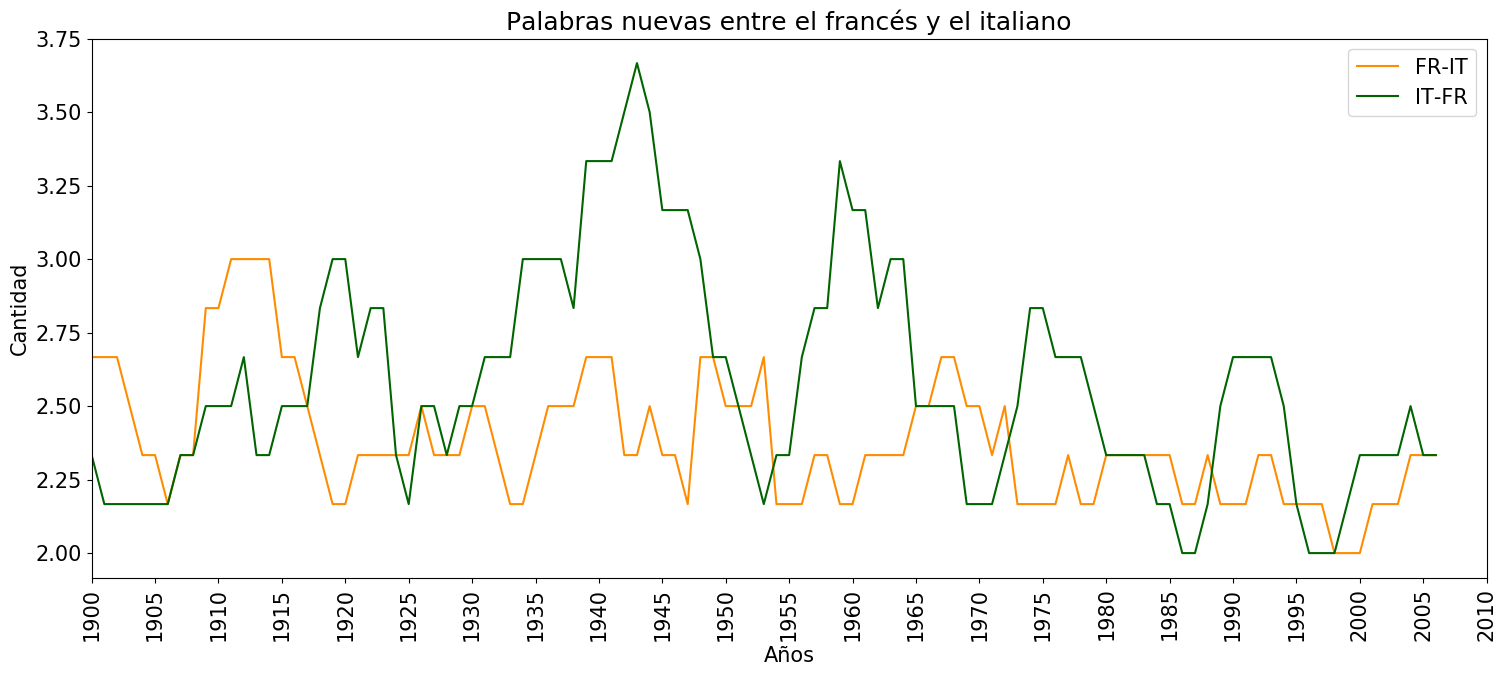
\includegraphics[scale=.38]{Cap_2/NC_3_S2_FR.png}
	\label{NC_FI}
	\caption{}
\end{figure}

La mayoría de los préstamos que ocurrieron entre estos idiomas provienen del italiano como el idioma origen, logrando puntos contrastantes con las migraciones provenientes del francés. Aunque países como Italia y Francia  fueron relevantes durante los años del análisis,  la mayoría de las palabras encontradas no brindan información para familiarizar a algún hecho,  en las pocas que se lograron conectar del francés al italiano están \textit{Versailles} y \textit{Poincaré} (1924) aludiendo al tratado de paz de la primera guerra mundial y al matemático francés.  También se encontró  \textit{Vietnam} (1966) y \textit{URSS} (1975), aunque no son términos franceses, si fue el francés el primero en hablar de ellos e importarlos a los demás idiomas.

En las migraciones con origen en el italiano, se encuentra \textit{Mussolini} (1935), la cual ya se había mencionado en las migraciones del italiano al inglés, tras revisar las listas de migraciones con origen italiano  a los demás idiomas, Mussolini siempre se encuentra en la lista de préstamos y con el mismo año de aparición en los demás idiomas.  Aunque solo sea una palabra, el estar en todos los idiomas del análisis ejemplifica la importancia de la misma en el siglo XX. 

\newpage
\subsection{Francés y Español}

\begin{figure}[h!]
	\centering
	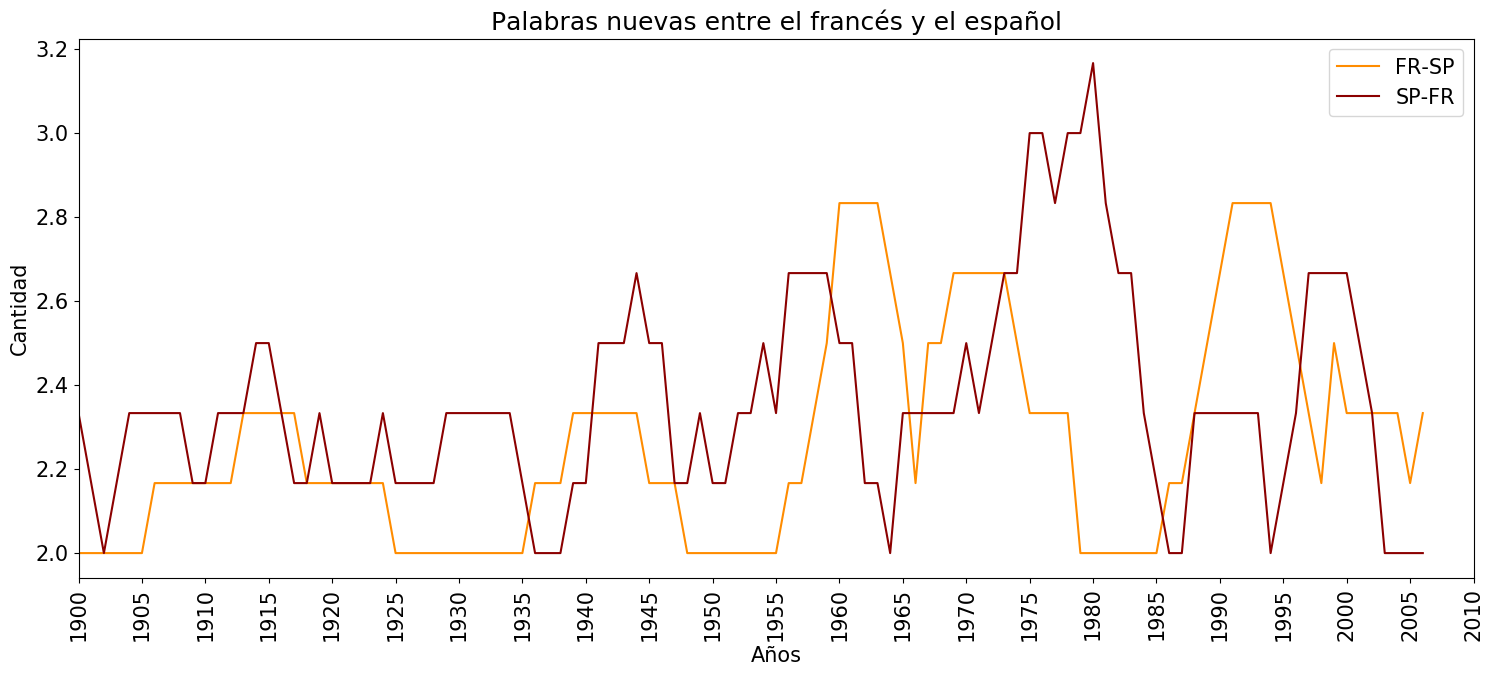
\includegraphics[scale=.38]{Cap_2/NC_4_S2_FR.png}
	\label{NC_FS}
	\caption{}
\end{figure}

La tendencia de los préstamos del español hacia el francés presentó pocos años donde la cantidad de ellos fue nula, en comparación con los del francés al español donde se aprecian periodos sin una migración.  Por parte de los préstamos con origen en el francés y receptor hay una ausencia de palabras que representen información de la época, la más relevante es \textit{euros}, referente a la moneda de la Unión Europea, ya que el año de aparición en el español y el año en el que empezó a circular de forma oficial coinciden, siendo el 2002.  La palabra \textit{ONU} (1995)  también se detectó en este sentido de migración; a pesar de ser la abreviación de  una organización mundial,  a la cual no se le puede asignar el francés como idioma origen, pero sí fue el francés el primer idioma ( entre los idiomas del trabajo)  en hablar de ella, y aunque la ONU tenga al español como uno de sus seis idiomas oficiales,  dentro de las publicaciones en español, la palabra ONU entró a la lista de las cinco mil más usadas  cincuenta años después de su fundación en 1945. Otras palabras encontradas son \textit{URSS} (1962) y  \textit{Vietnam} (1965),  las cuáles ya se habían mencionado en las anteriores migraciones del francés. 

El primer préstamo que resultó importante del español hacia el francés es \textit{Panamá}\,\,\, (1913), su trascendencia se liga al año de inauguración del canal de Panamá en 1914, siendo la obra una de las más importantes para el comercio de la época al conectar los océanos pacífico y atlántico, además el primer gobierno que impulsó económicamente la construcción del canal fue el francés,  aunque su conclusión y administración pasó a los Estados Unidos.  Las demás palabras incluidas las que migraron entre 1965 y 1985 no se logró identificar su relación con suceso  en el cual hayan sido importantes.

\hfill\break
\subsection{Alemán e Italiano}

\begin{figure}[h!]
	\centering
	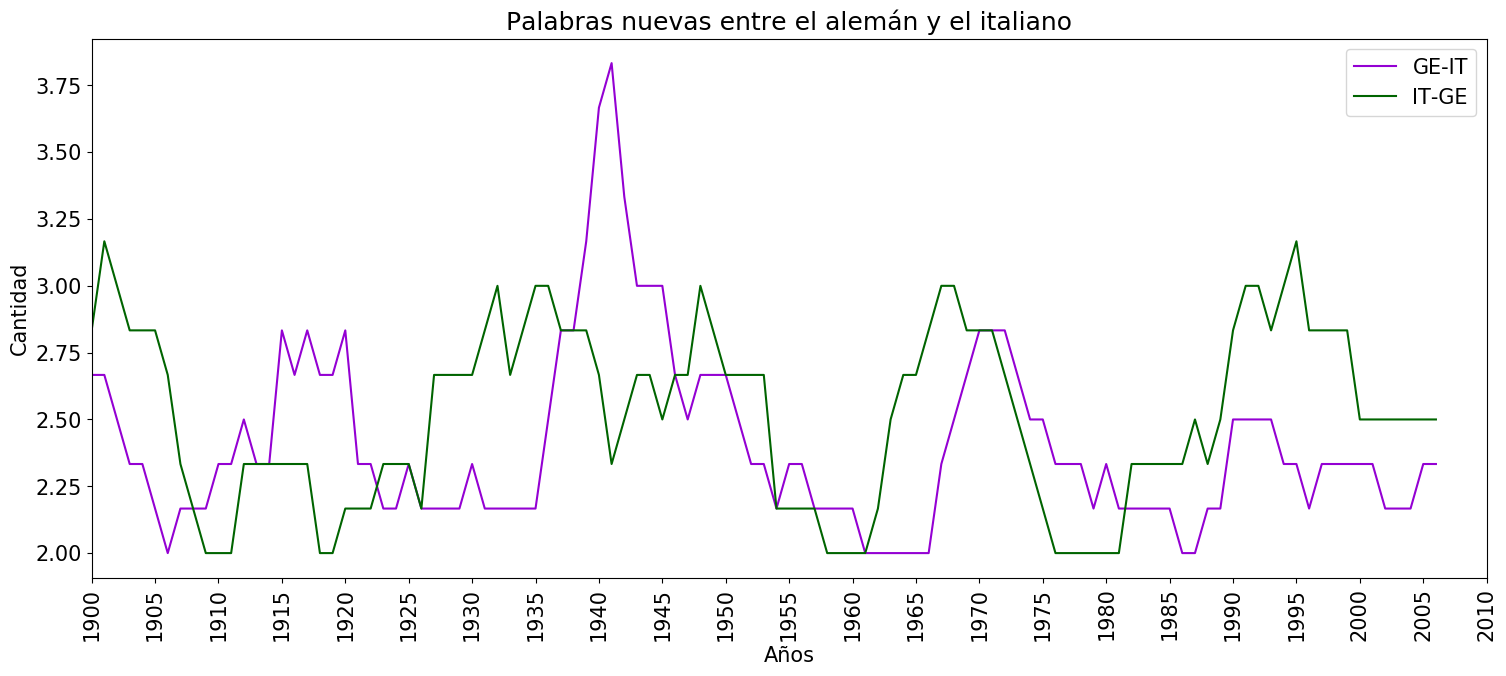
\includegraphics[scale=.38]{Cap_2/NC_3_S2_GE.png}
	\label{NC_GI}
	\caption{}
\end{figure}

La tendencia de las migraciones de palabras entre ambos idiomas se ve equitativa entre ambos idiomas,  siendo el punto más destacado alrededor de 1940 por parte del alemán como idioma origen. 

Tras la revisión de los préstamos del alemán hacia el inglés y el francés, se han destacado apellidos de personajes germano hablantes que destacaron en alguna disciplina. El apellido que se asentaron únicamente en el  italiano fue \textit{Berchtold} en 1943,  un año después de la muerte Leopold Berchtold (21 de noviembre de 1942) ministro de exteriores del Imperio Austro-Húngaro de 1912 a 1915, fecha coincidente con el inicio de la primera guerra mundial.  La relación entre la palabra y la fecha con los dos idiomas se puede explicar por las relaciones que tuvieron el imperio Austro-Húngaro con Italia, y además la parte germano parlante del imperio (actualmente Austria) tenía  fronteras con Italia, sumado a que una de las consecuencias de la primera guerra mundial fue la disolución del Imperio.  El argumento de las fronteras físicas entre países con diferentes idiomas oficiales, ejemplifica una de las posibles causas de la migración de palabras entre idiomas, ya que el intercambio cultural  y las relaciones entre ambas naciones pueden ser más activas o dinámicas permitiendo un mayor flujo de términos. 

Los préstamos del Italiano al Alemán permitieron relacionar con contextos bélicos de la época de la segunda guerra mundial a \textit{regime} (1938), \textit{panzer} (1941), \textit{duce} (1942),  traducciones de régimen, blindado y líder, además de \textit{Mussolini} (1935).  Uno de los errores que se encontró fue la palabra \textit{Franco} (1951), que por la fecha hace referencia al dictador español Francisco Franco; al ser un apellido, se registró como origen Italiano, pero mostrando como un término que es popular en un idioma diferente al origen, emigra a los demás idiomas  por un conjunto auxiliar.


\subsection{Alemán y Español}

\begin{figure}[h!]
	\centering
	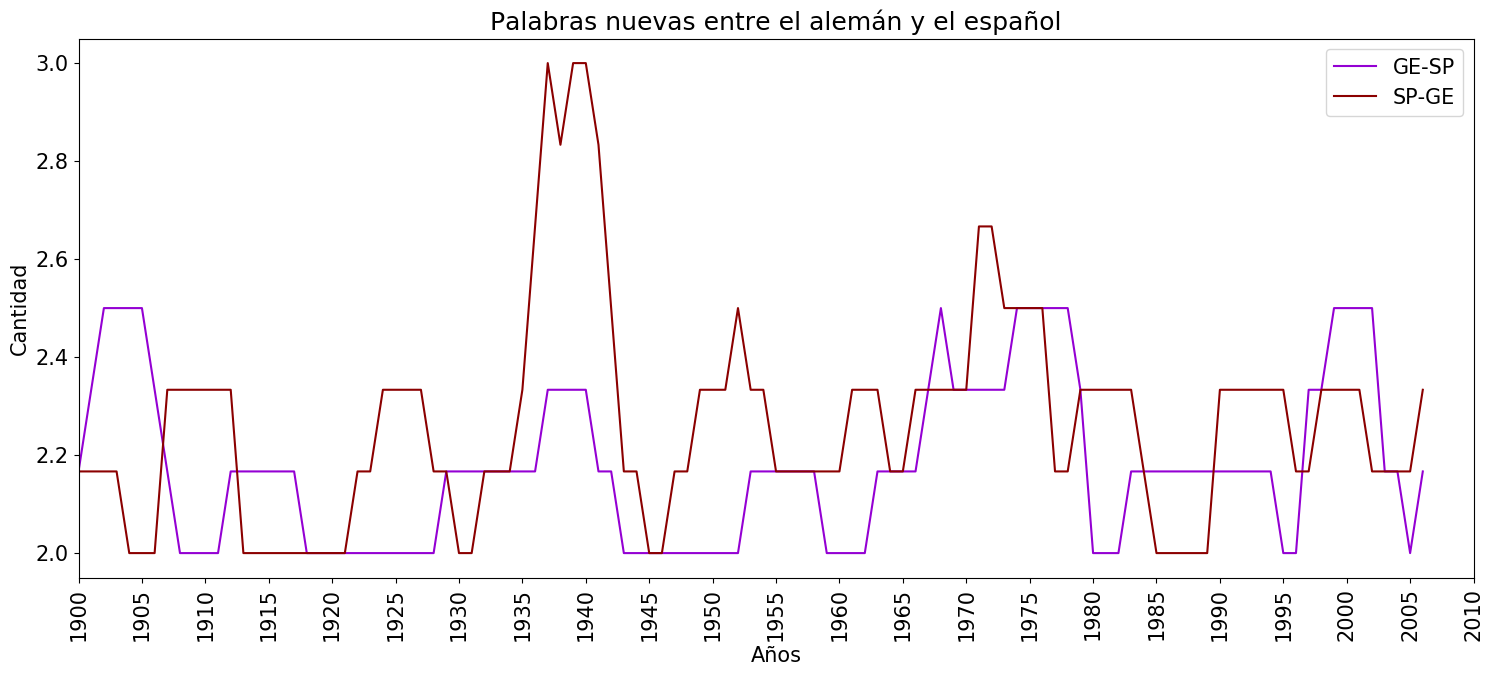
\includegraphics[scale=.38]{Cap_2/NC_4_S2_GE.png}
	\label{NC_GS}
	\caption{}
\end{figure}

La diferencia más marcada en las gráficas corresponde a las migraciones del español hacia el alemán entre 1930 y 1945, fechas que coinciden con el desarrollo de la segunda guerra mundial, sin embargo no se encontraron palabras que se relacionen con el evento.  La investigación hecha para ligar las palabras del español hacia el alemán con sucesos, muestra que la palabra \textit{lepra} (1901) fue globalmente importante a partir de 1874,  ya que en ese año el científico noruego Gerhard Armauer Hansen descubrió el bacilo de Hansen Mycobacterium Leprae \cite{lepra} que origina la enfermedad,  por el carácter médico de la palabra es probable que se hiciera más investigación sobre la enfermedad en diferentes idiomas, en este caso el alemán,  tras el descubrimiento del bacilo.  Este es otro caso de una palabra que se origina en un idioma (español), pierde  relevancia al transcurrir los años y tras un suceso (el descubrimiento del bacilo)  retoma importancia y migra a los demás idiomas (alemán).   Entre las otras palabras que pasaron al alemán están \textit{virus} (1939) que ya se ha tratado en los préstamos del español al inglés, \textit{China} (1955) referente al país y su relevancia en la segunda mitad del siglo XX por la revolución China de 1949, e \textit{India} (1970) igualmente se conecta con el país ya que en 1965 ocurrió la guerra indo-pakistaní,  también en 1968 hubo una extensa cobertura mediática a la banda británica The Beatles que visitó el norte de la India para meditar.

Las palabras que van en el sentido alemán-español,  presentaron muchos años sin una migración, el incremento de ellos se dio posterior a 1950  donde los años sin intercambio disminuyeron. En el contenido de la lista se encuentran palabras que ya se han tratado como \textit{Marx} (1932), \textit{kaiser} (1938), \textit{Hitler} (1940), \textit{Lenin} (1970), \textit{Hegel} (1971),  \textit{Nietzsche} (2000) y \textit{Freud} (2002).  Es peculiar que las dos últimas hayan aparecido en el español muchos años después que en los demás idiomas, por ejemplo en el francés Nietzsche apareció 1905 y Freud en 1965. El letargo de años puede ser una característica de el tiempo que les lleva  a las  palabras de un idioma  pasar hacia el español,  sobretodo si son palabras con un origen antiguo.

\hfill\break
\subsection{Italiano y Español}

\begin{figure}[h!]
	\centering
	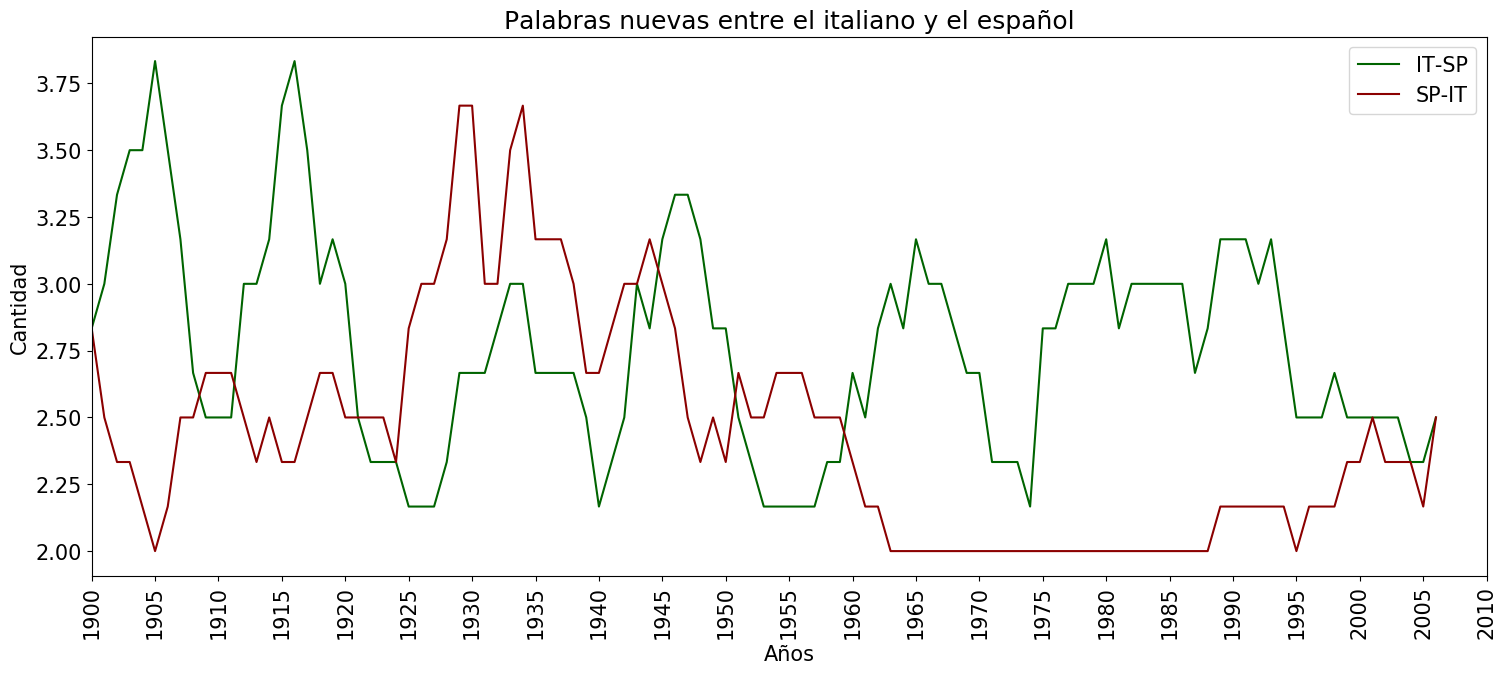
\includegraphics[scale=.38]{Cap_2/NC_4_S2_IT.png}
	\label{NC_IS}
	\caption{}
\end{figure}

Entre estos idiomas se dio la mayor cantidad de intercambios de palabras durante el siglo XX, durante la primera mitad, las aportaciones fueron equitativas con dos periodos donde dominó el italiano y dos donde dominó el español; a partir de 1960 el dominio fue italiano, ya que los aportes del español  fueron nulos hasta 1900. 

Por parte de los préstamos del italiano al español, se encuentran muchos con tendencias hacia ideologías políticas como \textit{socialista} (1914), \textit{comunista} (1932), \textit{capitalismo} (1935), \textit{fascismo} (1937),  \textit{marxismo} (1963) y \textit{terrorismo} (1986), palabras que por las fechas fueron importantes no solo en el italiano y el español, sino globalmente, ya que estas ideologías repercutieron en eventos como la guerra fría y la economía.  Una palabra que no se había tratado es realismo (1948) que tuvo un impulso por la corriente literaria del realismo mágico originado en varios países de Latinoamérica, cuyas obras trascendieron en la literatura. 

En las palabras que se originan en el español y llegan al italiano, se encontró \textit{idealismo} (1920) otra ideología política,  y palabras de términos médicos como \textit{virus} (1922), \textit{colesterina} (1928),  \textit{sintomatología} (1931), \textit{anestesia} (1932), \textit{vitamina} (1935), \textit{anemia}, \textit{metabolismo} y \textit{gástrica} en 1936  y \textit{endovenosa} (1937).  Este grupo de términos apareció en un periodo de veinte años, probablemente por la publicación de un texto que se popularizó, ya que muchas de estas palabras tienen su traducción al italiano. En los demás años, no se encontraron más palabras con un tema común al cual relacionar. 

\hfill\break
\hfill\break
\hfill\break
\section{Conclusiones del método}

El método de buscar préstamos nuevos mostró el diverso contenido de los préstamos que se lograron asociar un hecho,  por parte del inglés, las mayores aportaciones fueron apellidos de los presidentes de los Estados Unidos, y por el papel que tuvo este país en diferentes campos como la economía, la ideología política, el desarrollo industrial, la globalización y su participación en las grandes guerras, logró que sus jefes de estado fuesen relevantes en cada ámbito que se suscitó en la época que gobernaron.  Por parte del inglés como idioma receptor,  las palabras que emigraron al inglés, no exhibieron una tendencia clara sobre el campo al cual relacionarlas,  muchas de ellas son palabras con origen etimológico en el inglés pero que fueron más relevantes  en otros idiomas, antes de tomarlas como un error, estas palabras muestran que antes del siglo XX el inglés no tenía la importancia que actualmente posee, y que se apoyaba en otros idiomas para que sus vocablos fuesen conocidos. 

El Alemán fue otro conjunto donde los préstamos que llegan a otros idiomas se caracterizan por ser apellidos de personajes, a diferencia del inglés, los campos donde destacaron los germanoparlantes fueron ciencias, filosofía, medicina y  por la historia de alemania en las guerras mundiales,  palabras de carácter bélico también migraron a los distintos receptores.

El francés, aportó endónimos a los otros idiomas, principalmente en las primeras décadas del siglo, reflejando la importancia que tuvo este idioma en el siglo XIX y principios del XX, al migrar palabras que tienen su propio significado y escritura en los demás idiomas.  Además de endónimos,  una porción significativa de los aportes son palabras etimológicas del inglés,  este punto ya fue discutido, pero es otra muestra de la relación que ha mantenido el inglés y el francés  desde antes de 1800, al tener el inglés muchas palabras provenientes de la familia del francés, es decir las lenguas grecolatinas. 

El italiano migró términos políticos a los demás idiomas, principalmente al español,  mientras que el español fue diverso en el contenido de sus préstamos,  desde expresiones médicas, nombres de países y  literatura. La diversidad del español se puede deber a la cantidad de países donde es un idioma oficial,  y hay muchos elementos de diferentes culturas que se exportan a los demás idiomas. 

Tanto el francés, el alemán, el italiano y el español,  se comportaron más como idiomas receptores que como portadores,  donde la mayoría de palabras provienen del inglés.  Entonces en términos de cantidad, el inglés ha sido el idioma que más ha influenciado a los demás, por los vocablos nuevos que de él han llegado.  


En términos de préstamos nuevos,  la influencia por cantidad mostró información histórica de los países en el siglo pasado,  pero no el cómo afectan las nuevas palabras a los idiomas receptores. Si los préstamos nuevos cobran relevancia en el idioma receptor, el rango que ocupan disminuye en cada lista tras el año en que se localizaron,  sin embargo se encontraron años donde no hay préstamos nuevos, y al ser pocos en comparación a las cinco mil palabras, su frecuencia de uso, ecuación \ref{ec.fuso} es casi nula, por ello la mejor forma de utilizar a la frecuencia de uso es usando el background de préstamos acumulados. 
















	